\documentclass{article}

% Language setting
% Replace `english' with e.g. `spanish' to change the document language
\usepackage[english]{babel}

% Set page size and margins
% Replace `letterpaper' with `a4paper' for UK/EU standard size
\usepackage[letterpaper,top=2cm,bottom=2cm,left=3cm,right=3cm,marginparwidth=1.75cm]{geometry}

% Useful packages
\usepackage{amsmath}
\usepackage{graphicx}
\usepackage[colorlinks=true, allcolors=blue]{hyperref}

\title{HW4}
\author{Xicheng Li\\xl657\\section2}

\begin{document}
\maketitle

All commands and corresponding instructions are in the ReadMe.txt of HW4

\section{Question 1}

\subsection{}

\textbf{My Approach and reasoning:}

First, for data preprocessing, because the input is 32×32, the 28×28 MNIST must be padded with zero borders. export-data.py expands the original MNIST 28×28 grayscale image by 2 pixels, saves it as 32×32 PNG, and writes the corresponding label file.
\\
Secondly, prepare-rbf.py scales all images of the same digit in the training set to 12×7 and averages them when RBF output is needed, generating 10 "template vectors" (rbf-centers.pt).
\\
Then, lenet5.py is the construction of the model. Three layers of convolution are used to obtain 120-dimensional features, followed by a layer of full connection. The convolutional layer extracts local features and reduces the number of parameters through weight sharing.
\\
Subsequently, there are two options for the output layer:
Linear layer Linear(84,10) - directly generates 10 category scores;
RBF layer - uses the above template to calculate the negative square distance to the center of each category; It uses the average image of each class as the center, the model finally compares "distance" instead of linear weights.
\\
Finally, the ReLU activation function is used between convolution blocks.
\\
train.py is the file for training the model. The input is divided by 255 and then linearly mapped to [-1,1]. Iterate with batch size 64, and use Adam (lr=1e-3) as optimizer.
If linear output is used, the loss is Cross‑Entropy; if RBF output is used, the loss is Equation 9 in the paper. The error rate of the entire set of training/test images is counted and printed for each epoch. After training, save the model and draw the error curve.
\\
test1.py is the test file. I added LeNet5 to the whitelist at the beginning and temporarily changed torch.load to the old behavior. I use weights-only=True to prevent malicious pickling, while keeping the old full deserialization capabilities intact via manual whitelisting and monkey‑patch.


\subsection{}
Error rate at each iteration:
\begin{tabular}{c c c}
Epoch & train error & test error \\
1  & 0.0948 & 0.0279 \\
2  & 0.0272 & 0.0204 \\
3  & 0.0193 & 0.0147 \\
4  & 0.0158 & 0.0112 \\
5  & 0.0132 & 0.0103 \\
6  & 0.0116 & 0.0111 \\
7  & 0.0098 & 0.0114 \\
8  & 0.0085 & 0.0100 \\
9  & 0.0077 & 0.0103 \\
10 & 0.0068 & 0.0116 \\
11 & 0.0055 & 0.0117 \\
12 & 0.0055 & 0.0097 \\
13 & 0.0046 & 0.0090 \\
14 & 0.0041 & 0.0091 \\
15 & 0.0038 & 0.0080 \\
16 & 0.0036 & 0.0100 \\
17 & 0.0031 & 0.0101 \\
18 & 0.0028 & 0.0117 \\
19 & 0.0030 & 0.0081 \\
20 & 0.0030 & 0.0104 \\
\end{tabular}


\subsection{}
\textbf{test accuracy: 0.9330}
\begin{figure}[htbp]
  \centering
  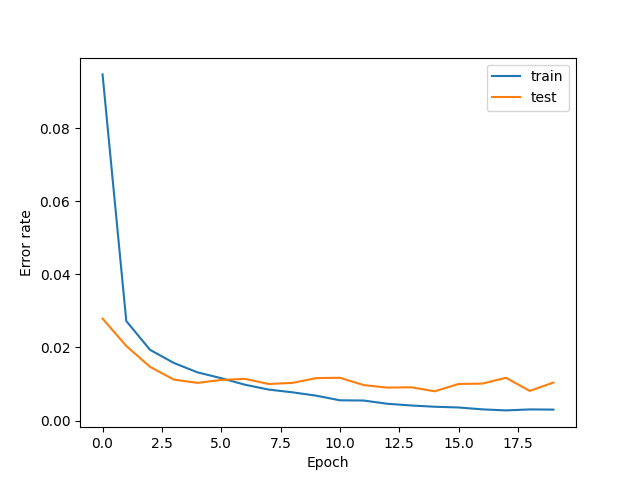
\includegraphics[width=0.7\textwidth]{error_plot.png} 
  \caption{plot of training and test error rate}
  \label{fig:example}
\end{figure}

error rates:
\\train error rate at epoch 20 is 0.3% 
\\test error rate at epoch 20 is 1.04%
\\
\\
Digit 0: test‑idx  6597 was misclassified with the highest confidence, it misclassified‑as 9\\
Digit 1: test‑idx  4507 was misclassified with the highest confidence, it misclassified‑as 9\\
Digit 2: test‑idx  4176 was misclassified with the highest confidence, it misclassified‑as 7\\
Digit 3: test‑idx  2927 was misclassified with the highest confidence, it misclassified‑as 2\\
Digit 4: test‑idx  2130 was misclassified with the highest confidence, it misclassified‑as 9\\
Digit 5: test‑idx  2597 was misclassified with the highest confidence, it misclassified‑as 3\\
Digit 6: test‑idx  2654 was misclassified with the highest confidence, it misclassified‑as 1\\
Digit 7: test‑idx  1226 was misclassified with the highest confidence, it misclassified‑as 2\\
Digit 8: test‑idx  1878 was misclassified with the highest confidence, it misclassified‑as 3\\
Digit 9: test‑idx  1901 was misclassified with the highest confidence, it misclassified‑as 4\\
\\
\\
confusion matrix: \\
\begin{tabular}{l c c c c c c c c c c}
        & Pred 0 & Pred 1 & Pred 2 & Pred 3 & Pred 4 & Pred 5 & Pred 6 & Pred 7 & Pred 8 & Pred 9 \\
\hline
True 0  &   977  &     1  &     0  &     0  &     0  &     0  &     1  &     0  &     0  &     1  \\
True 1  &     0  &  1131  &     1  &     0  &     0  &     1  &     0  &     0  &     1  &     1  \\
True 2  &     1  &     1  &  1027  &     0  &     1  &     0  &     0  &     1  &     1  &     0  \\
True 3  &     0  &     1  &     6  &   998  &     0  &     2  &     0  &     0  &     2  &     1  \\
True 4  &     0  &     0  &     0  &     0  &   979  &     0  &     0  &     0  &     0  &     3  \\
True 5  &     2  &     0  &     0  &     5  &     0  &   883  &     1  &     0  &     1  &     0  \\
True 6  &     4  &     3  &     1  &     0  &     2  &     5  &   942  &     0  &     1  &     0  \\
True 7  &     0  &     5  &    14  &     0  &     0  &     0  &     0  &  1002  &     1  &     6  \\
True 8  &     0  &     0  &     2  &     3  &     0  &     2  &     2  &     1  &   962  &     2  \\
True 9  &     0  &     0  &     2  &     0  &     8  &     2  &     0  &     1  &     1  &   995  \\
\end{tabular}




\section{Question 2}

\subsection{}
\textbf{Plan and explanation:}
\\
LeNet2 retains the convolutional framework of LeNet1. However, it is modified at the input, feature extraction, and training ends to improve robustness to geometric perturbations and handwriting style differences.
First, for the input, I made changes in rotation, translation, and size. This prepares the model during the training phase. This symmetric normalization makes ReLU not biased to one side and makes the gradient more stable.
Second, for the network body, I used Spatial Transformer Network to reduce the burden of subsequent convolutions. STN provides continuous and learnable geometric correction, allowing the model to remain adaptable to deformations beyond the range of random enhancement. MaxPool selects strong texture responses to resist noise. MaxPool takes the maximum value of 4 pixels and leaves the main body of the stroke. This is naturally more robust to noise. Dropout randomizes joints to reduce dependence on specific text styles. This alleviates overfitting. Dropout and weight decay suppress overfitting.
Finally, for training, I used SGD, Momentum 0.9, and CosineAnnealing. This allows momentum to converge faster without oscillation. At the same time, Cosine scheduling searches roughly at the beginning but fine-tunes little by little in the later stages. This allows the model to achieve lower validation error within the same epoch.

train error and validation error in the first 20 epochs: 
\begin{tabular}{c c c}
Epoch & train\_err & val\_err \\
1  & 0.0899 & 0.0369 \\
2  & 0.0565 & 0.0288 \\
3  & 0.0426 & 0.0199 \\
4  & 0.0360 & 0.0194 \\
5  & 0.0336 & 0.0226 \\
6  & 0.0315 & 0.0169 \\
7  & 0.0266 & 0.0144 \\
8  & 0.0239 & 0.0132 \\
9  & 0.0247 & 0.0120 \\
10 & 0.0205 & 0.0129 \\
11 & 0.0199 & 0.0115 \\
12 & 0.0151 & 0.0114 \\
13 & 0.0218 & 0.0106 \\
14 & 0.0147 & 0.0092 \\
15 & 0.0127 & 0.0107 \\
16 & 0.0114 & 0.0085 \\
17 & 0.0112 & 0.0090 \\
18 & 0.0106 & 0.0081 \\
19 & 0.0104 & 0.0072 \\
20 & 0.0103 & 0.0063 \\
\end{tabular}

Validation error measures the performance of the model on unseen data.

\end{document}